% !TEX encoding = UTF-8 Unicode
\chapter{Trabajos relacionados}
\label{chap:trabajos_relacionados}
%
%
A continuación se hará una revisión de algunos trabajos relevantes para la presente investigación.
Como se detallará, existen propuestas que abordan problemas similares al que se plantea en este trabajo; sin embargo, estos se abordan de maneras distintas a la que se propone en esta tesis.
De entre ellos se pueden mencionar los siguientes: 
%
\begin{itemize}
	\item El problema de acomodar objetos en un contenedor, problema de carga del contenedor o \textit{bin-packing problem}, por su denominación en inglés \cite{doi:10.1287/opre.48.2.256.12386}\cite{10.5555/98124}.
	\item El problema de tomar objetos de un contenedor o \textit{bin picking problem}, por su denominación en inglés \cite{1699272}.
	\item Los NAMO (\textit{Navigation Among Movable Obstacles}, por sus siglas en inglés) \cite{doi:10.1142/S0219843605000545}.
	\item Los MAMO (\textit{Manipulation Among Movable Obstacles}, por sus siglas en inglés) \cite{4209604}.
	\item El problema de reordenamiento o \textit{rearrangement problem}, por su denominación en inglés.
\end{itemize}
%
%
% Problema del contenedor
%
%
El problema de carga del contenedor, referido en adelante como problema del contenedor, consiste en colocar un conjunto de objetos en uno o más contenedores, de manera que el volumen total ocupado por dichos objetos se minimize. 
Para acercar el problema más a la realidad, se pueden agregar algunas restricciones adicionales, por ejemplo, se puede tomar en cuenta el peso de los objetos, su orientación, su separación, la prioridad de envío, etc. \cite{BISCHOFF1995377}. 

Es relativamente común encontrarse con este problema, sobre todo en ámbitos relacionados con el comercio o la industria, por lo cual, se han propuesto diversos enfoques para su solución.

En \cite{GONCALVES2012179} se propone un algoritmo para administrar los espacios libres en el problema del contenedor, el cual integra un algoritmo genético de clave aleatoria sesgada de múltiples poblaciones.
Su proceso genera una lista de espacios máximos en el contenedor cada vez que un nuevo elemento es colocado, tal y como se muestra en la Figura \ref{fig:GONCALVES2012179}.
Posteriormente, se intenta colocar uno o varios elementos nuevos en los espacios vacíos.
Los autores utilizan dos variantes de este enfoque: uno en el cual los espacios vacíos tienen soporte completo por debajo y otro donde no lo tienen. 
El espacio en el cual se colocará un nuevo elemento se selecciona mediante una heurística basada en arreglos rectangulares de cajas del mismo tipo, llamados \textsl{capas}.
Cada vez que una capa es colocada en el contenedor se generan nuevos \textsl{espacios máximos}.
Los resultados muestran una mejora respecto a trabajos previos en la literatura.
%
\begin{figure}[H]
	\begin{subfigure}{0.22\linewidth}
		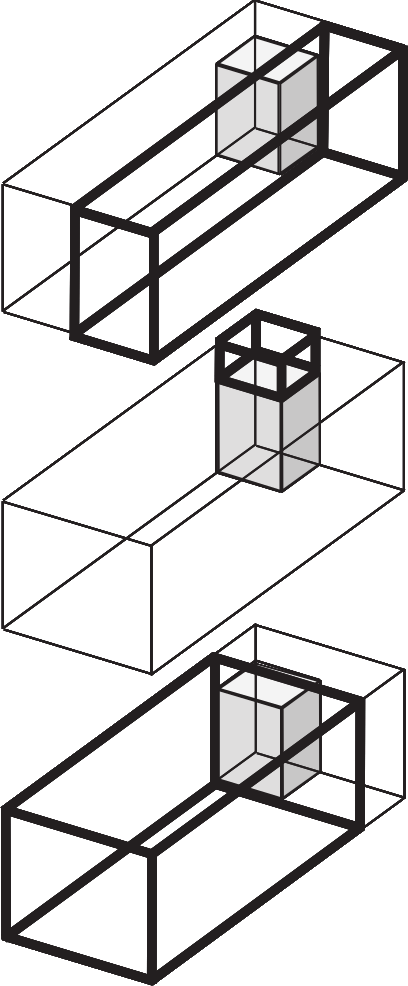
\includegraphics[width=\linewidth]{jose_fernando_a}%
		\label{subfig:con_soporte}%
	\end{subfigure}%
	%
	\hspace{1.8cm}%
	%
	\begin{subfigure}{0.22\textwidth}
		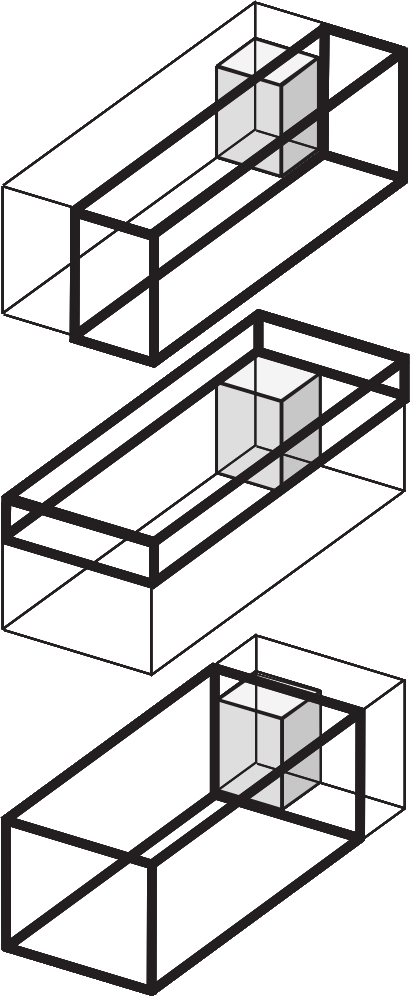
\includegraphics[width=\linewidth]{jose_fernando_b}%
		\label{subfig:sin_soporte}%
	\end{subfigure}%
	%
	\caption{Espacios máximos generados: con soporte (izquierda) y sin soporte (derecha) por debajo (imágenes tomadas de \cite{GONCALVES2012179}).}%
	\label{fig:GONCALVES2012179}%
\end{figure}
%
En \cite{BORTFELDT2001143} se presenta un algoritmo genético para resolver el problema de un solo contenedor, aplicando varias de las restricciones mencionadas en \cite{BISCHOFF1995377}; algunas de las cuales son: la orientación de los paquetes, la estabilidad de paquetes que no son colocados directamente en el suelo, y finalmente, la de no colocar paquetes encima de otros bajo circunstancias específicas.
Para este propósito, se utiliza una estructura de capas para acomodar los objetos, la cual consiste en agregar paredes internas al contenedor, de forma que los espacios generados por estas paredes sean llenados de forma codiciosa.
Los resultados obtenidos en este artículo muestran ser mejores que los de otros métodos con los que se comparan.

De forma similar en \cite{1492318} se presenta un algoritmo para la solución del problema del contenedor. 
En este se incluyen tres restricciones: orientación de las cajas, estabilidad de la carga y volumen del contenedor. 
Dicho algoritmo está basado en el paradigma de búsqueda aleatoria adaptativa codiciosa y está evaluado en términos de las restricciones mencionadas y la comparación con otros nueve algoritmos.
La heurística que utilizan se basa en el concepto de espacio vacío: una región con forma de paralelepípedo en la cual ninguna caja ha sido colocada.

El algoritmo utilizado considera todas las orientaciones y posiciones posibles de una caja y selecciona el arreglo cuyo uso del volumen en el contenedor sea menor.
Los autores mencionan que su enfoque produce soluciones que superan las de otros en términos de la máxima ocupación del volumen disponible y estabilidad de la carga.

En \cite{10.1145/2816795.2818064} se muestra una solución al problema del contenedor aplicado en la impresión de modelos 3D; cómo los que se muestran en la Figura \ref{fig:10.1145/2816795.2818064}. 
Para ello se realiza una partición de un objeto 3D que se desea imprimir, de manera que se puedan acomodar las piezas en un contenedor de espacio mínimo. 
Con esto se busca economizar espacio y tiempo de producción. 
%
\begin{figure}[H]
	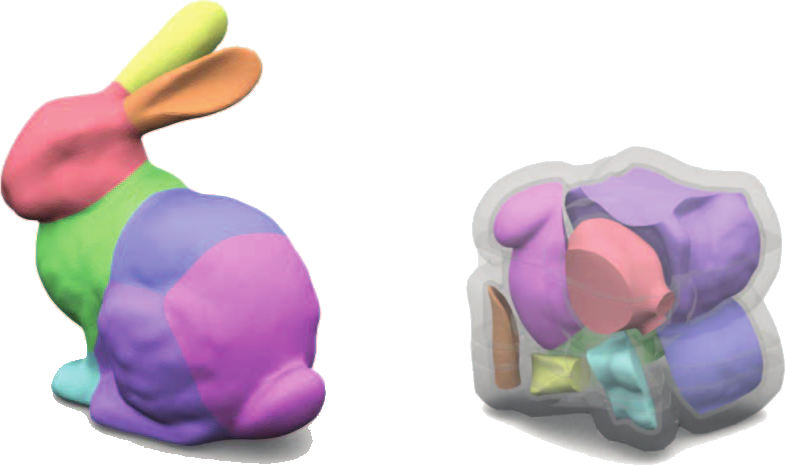
\includegraphics[height=3.3cm]{yao_miaojun_a}%
	\hspace{1cm}%
	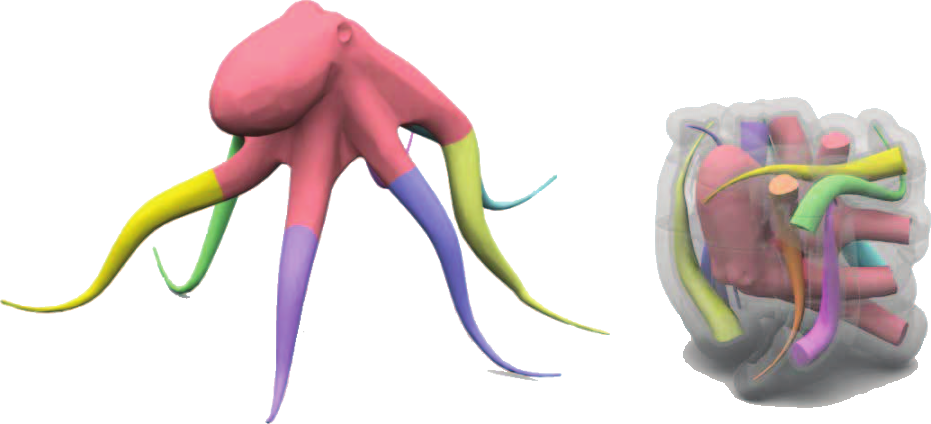
\includegraphics[height=3.3cm]{yao_miaojun_b}%
	%
	\caption{Ejemplos de segmentado y acomodo de figuras 3D (imágenes tomadas de \cite{10.1145/2816795.2818064}).}%
	\label{fig:10.1145/2816795.2818064}%
\end{figure}
%
Una de las características en común del problema del contenedor con respecto al planteado en este trabajo, es que no se tiene certeza del arreglo de objetos al que se va a llegar. 
Por un lado, mientras que el interés principal del problema del contenedor es asegurar la máxima ocupación del volumen disponible, para de esa forma poder colocar el mayor número de objetos posible en él; en el problema propuesto se da por hecho que todos los objetos disponibles caben en el espacio utilizable, por lo que no hay restricciones sobre la ocupación de este.

El problema de tomar objetos de un contenedor o \textit{bin-picking problem}, se refiere al problema para el cual un robot o manipulador debe tomar un objeto de un contenedor de forma automática. 
El problema en su forma general, tiene como característica principal que los objetos están colocados de forma aleatoria en un contenedor de dimensiones conocidas.

Este problema hasta la fecha no tiene solución.
Esto debido principalmente a cuestiones de oclusión en los objetos \cite{1699272}, donde, por causa de obstrucciones entre objetos o ruido en los datos, no todas las características de los objetos son visibles al mismo tiempo por las cámaras u otros sistemas de visión, dificultando la estimación de la posición y orientación de los objetos. 

El problema de tomar objetos de un contenedor representa un gran reto para la robótica, debido a que en él se involucran diversos sub-problemas que requieren un alto dominio de diferentes técnicas de la robótica y la inteligencia artificial.
Entre estas técnicas se pueden mencionar la adquisición de datos \cite{CHEN1992145}, la localización y estimación de la posición y orientación de un objeto \cite{5152739} o la prevención de colisiones \cite{6239716}\cite{5756828}.
Sin embargo, debido a que se trata de un tema importante para la industria, se han realizado varios esfuerzos por resolverlo; algunos de los cuales hacen una reducción de su complejidad al tratar solo instancias específicas.

En \cite{5756828} se utiliza un robot industrial para resolver instancias particulares del problema de tomar objetos de un contenedor.
El robot en este trabajo está equipado con un sistema de visión 3D y un efector final, que puede ser una pinza estándar o una pinza de vacío, dependiendo del tipo de objeto que se vaya a manipular.
El sistema de visión se utiliza para calcular la posición de un objeto, así como para detectar de forma general si este se puede sujetar.
Después de esto, se hace el plan de una trayectoria libre de colisiones hacia el objeto y este es tomado.
Finalmente, el objeto es insertado en una estación de proceso de forma muy precisa y con una orientación particular.
Se realizaron experimentos con tuercas como objetos de prueba, tal como se muestra en la Figura \ref{fig:5756828}.
Como se demuestra, el robot es capaz de tomar todas las tuercas del contenedor.
%
\begin{figure}[H]
	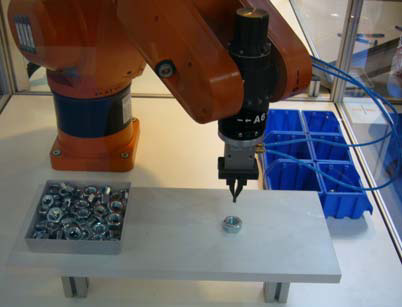
\includegraphics[width=7cm]{a_pochyly}%
	\caption{Configuración experimental para la toma de tuercas de un contenedor con un brazo robótico (imagen tomada de \cite{5756828}).}%
	\label{fig:5756828}%
\end{figure}
%
En \cite{8793966} se presenta una solución a la combinación de dos problemas: el problema de tomar objetos de un contenedor y el problema del contenedor.
El problema consiste en tomar objetos en desorden de un contenedor $A$ y acomodarlos en otro contenedor $B$, tal como se muestra en la Figura \ref{fig:8793966}, intentando maximizar el número de objetos en este último.
Para esto se utiliza un brazo robótico con una pinza de vacío que utiliza únicamente imágenes de profundidad para sensar su ambiente.

La pinza del brazo robótico, además de usarse para trasladar objetos de un lugar a otro, también es utilizada para empujarlos cuando se encuentran dentro del contenedor $B$.
Esto con el objetivo de hacer pequeñas correcciones a sus posiciones, haciendo al arreglo más compacto.
Asimismo, se utiliza una función para reconfigurar los objetos dentro del contenedor $A$, al derribarlos para poder tomarlos de una forma apropiada.

Debido a que todos los objetos manipulables tienen forma de prisma rectangular, la forma del arreglo que se busca para el contenedor $B$ es en forma de malla.
Finalmente, se realizan diversas pruebas con un brazo real, en las que se muestra la dependencia de las funciones para derribar y empujar objetos sobre el arreglo final en $B$.
%
\begin{figure}[H]
	\begin{subfigure}{0.45\linewidth}
		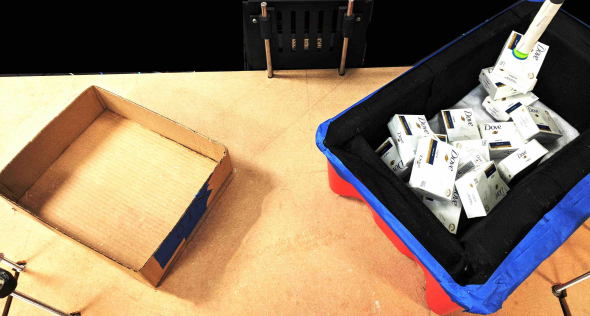
\includegraphics[width=\linewidth]{rahul_shome_kiril_solovey_a}%
		\label{subfig:bin_picking_dove_a}%
	\end{subfigure}%
	%
	\hspace{0.5cm}%
	%
	\begin{subfigure}{0.45\linewidth}
		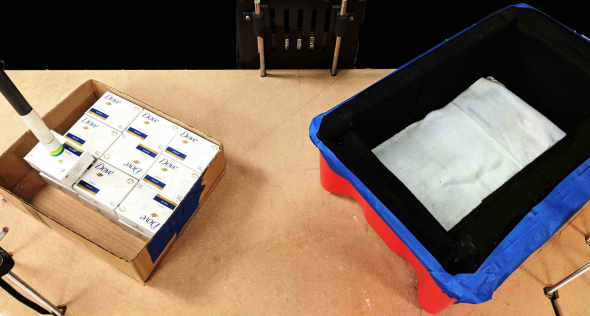
\includegraphics[width=\linewidth]{rahul_shome_kiril_solovey_b}%
		\label{subfig:bin_picking_dove_b}%
	\end{subfigure}%
	%
	\caption{Configuración de objetos: antes (izquierda) y después (derecha) de la intervención del brazo robótico (imágenes tomadas de \cite{8793966}).}%
	\label{fig:8793966}%
\end{figure}
%
En \cite{doi:10.1177/0278364911436018} se presenta un sistema basado en visión para tratar el problema de tomar objetos de un contenedor.
Este sistema es capaz de lidiar con sub-problemas relacionados con la caracterización de materiales, problemas de ambiente (polvo, grasa, etc.), estimación de la posición y orientación de los objetos, entre otros.

En este trabajo se presenta un algoritmo de correspondencia de forma; el cual es usado para detectar los objetos de manera confiable.
Para la sujeción de objetos se utiliza un brazo robótico real, que toma los objetos del contenedor y realiza un refinamiento de la posición y orientación del objeto mientras este se encuentra en la pinza. 
También se utiliza una cámara multi-flash, con la cual se detectan los bordes de los objetos con una mayor facilidad.

Se realizaron pruebas de detección con objetos reales, en las cuales el sistema de visión es capaz de reconocer varios objetos de formas complejas, los cuales se encuentran desordenados en el contenedor, tal y como se muestra en los diferentes ejemplos de la Figura \ref{fig:doi:10.1177/0278364911436018}.
El sistema es capaz de detectar y estimar de manera precisa la pose de objetos con reflejos especulares (como se muestra en las Figuras \ref{subfig:bin_picking_a} a \ref{subfig:bin_picking_d}); así como objetos sin una textura definida (Figura \ref{subfig:bin_picking_e}); o bien objetos pintados con una textura engañosa (Figura \ref{subfig:bin_picking_f}).
En los experimentos que realizan los autores se logra un porcentaje de eficiencia en la toma de objetos del 94\!\%.
%
\begin{figure}[H]
	\def\hsep{4pt}%
	\begin{subfigure}{0.32\linewidth}
		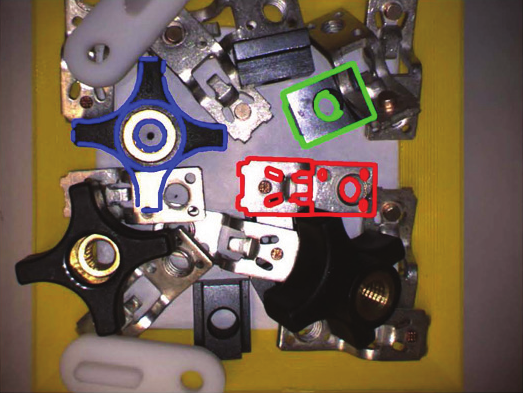
\includegraphics[width=\linewidth]{liu_ming_yu_a}%
		\subcaption{}%
		\label{subfig:bin_picking_a}%
	\end{subfigure}%
	\hspace{\hsep}%
	\begin{subfigure}{0.32\linewidth}
		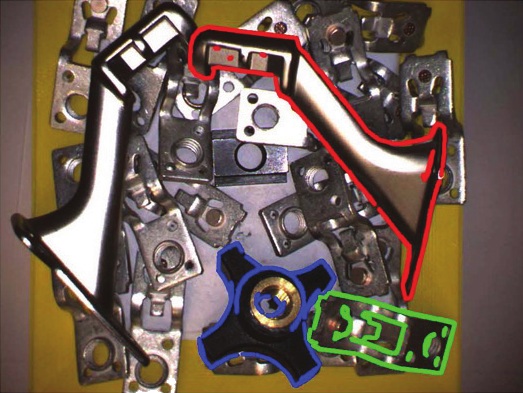
\includegraphics[width=\linewidth]{liu_ming_yu_b}%
		\subcaption{}%
		\label{subfig:bin_picking_b}%
	\end{subfigure}%
	\hspace{\hsep}%
	\begin{subfigure}{0.32\linewidth}
		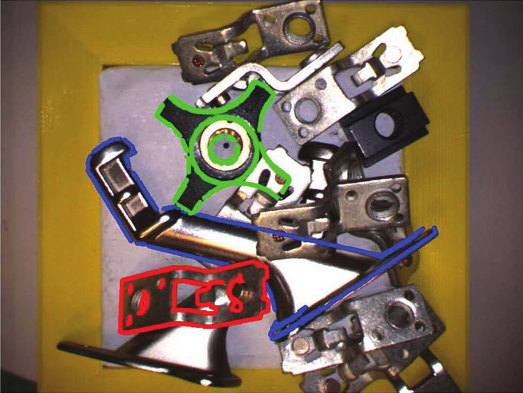
\includegraphics[width=\linewidth]{liu_ming_yu_c}%
		\subcaption{}%
		\label{subfig:bin_picking_c}%
	\end{subfigure}%
	
	\vspace{3pt}	
	
	\begin{subfigure}{0.32\linewidth}
		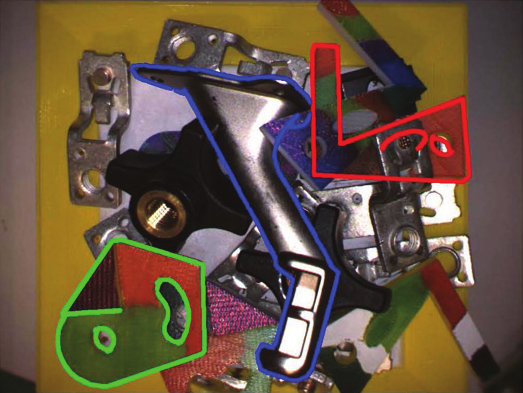
\includegraphics[width=\linewidth]{liu_ming_yu_d}%
		\subcaption{}%
		\label{subfig:bin_picking_d}%
	\end{subfigure}%
	\hspace{\hsep}%
	\begin{subfigure}{0.32\linewidth}
		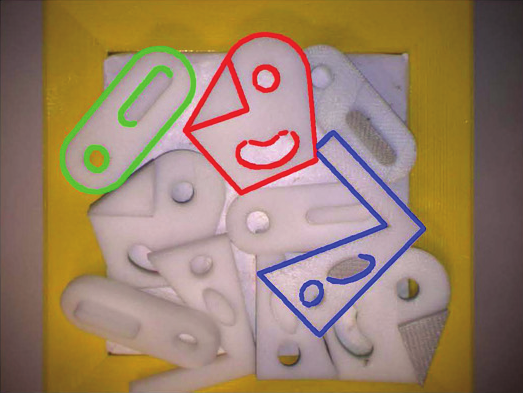
\includegraphics[width=\linewidth]{liu_ming_yu_e}%
		\subcaption{}%
		\label{subfig:bin_picking_e}%
	\end{subfigure}%
	\hspace{\hsep}%
	\begin{subfigure}{0.32\linewidth}
		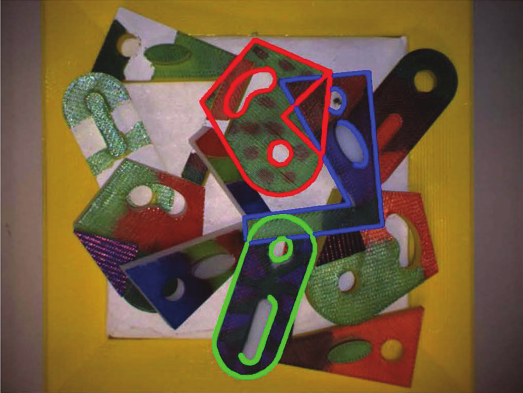
\includegraphics[width=\linewidth]{liu_ming_yu_f}%
		\subcaption{}%
		\label{subfig:bin_picking_f}%
	\end{subfigure}%
	%
	\caption{Detección de objetos desordenados en un contenedor (imágenes tomadas de \cite{doi:10.1177/0278364911436018}).}%
	\label{fig:doi:10.1177/0278364911436018}%
\end{figure}%
%
En \cite{pmlr-v78-mahler17a} se propone un método que modela el problema de tomar objetos de un contenedor con un Proceso de Decisión de Markov Parcialmente Observable de tiempo discreto.
Dicho método toma como entrada nubes de puntos de los objetos, obtenidas por una cámara de profundidad, como se muestra en la Figura \ref{subfig:depth_image}; y como salida entrega una posición y orientación del efector final para remover un objeto que se encuentra inmerso en un conjunto de objetos desordenados.
También se hace uso de un supervisor algorítmico, el cual realiza un cómputo previo de un conjunto de agarres robustos para cada objeto, utilizando la información disponible acerca de estos.
A partir de esto, se generan demostraciones sintéticas de agarre para el robot.

Los autores consideran una acción como el proceso completo de mover la pinza hacia el objeto, cerrarlo para sujetarlo y levantarlo.
Además, utilizan una simulación dinámica de varios cuerpos para determinar el siguiente estado de los objetos después de tomar uno, así como para determinar si un objeto puede ser levantado o no.

Se realizan experimentos en un robot real utilizando diferentes niveles de ruido en los datos de entrenamiento.
Para esto, se utiliza un conjunto de 50 objetos de diferentes formas y tamaños, mostrados en la Figura \ref{subfig:fifty_objects}, los cuales tienen que ser trasladados desde un contenedor a otro, tal como se muestra en la Figura \ref{subfig:object_picking}.
El robot debe agarrar objetos del contenedor señalado con borde verde y dejarlos en el contenedor con el borde azul.
Sus resultados muestran una tasa aceptable de éxito del 94\!\% en los intentos de mover un objeto de un contenedor a otro.
%
\begin{figure}[H]
	\begin{subfigure}[t]{0.275\linewidth}
		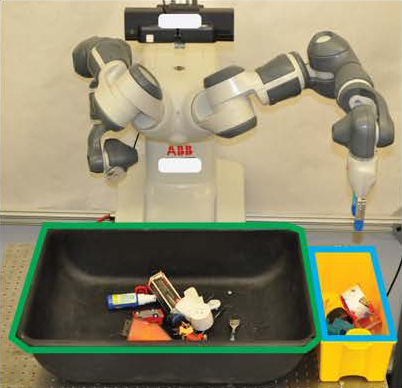
\includegraphics[height=4cm]{jeffrey_mahler_a}%
		\subcaption{}%
		\label{subfig:object_picking}%
	\end{subfigure}%
	\hspace{10pt}%
	\begin{subfigure}[t]{0.45\linewidth}
		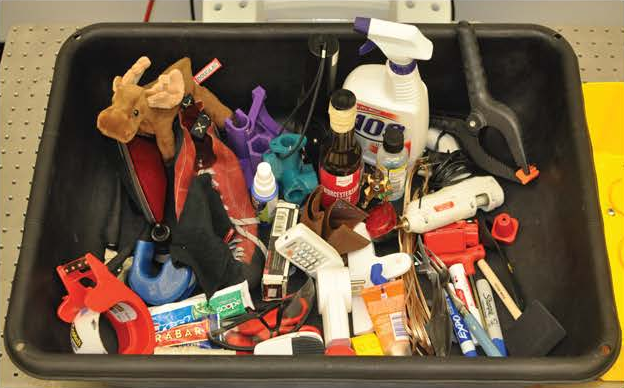
\includegraphics[height=4cm]{jeffrey_mahler_b}%
		\subcaption{}%
		\label{subfig:fifty_objects}%
	\end{subfigure}%
	%
	\begin{minipage}[b][4cm]{3.2cm}%
	\begin{subfigure}[t]{\linewidth}
		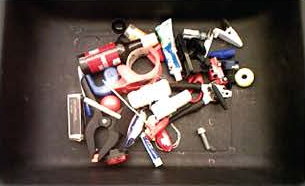
\includegraphics[width=3.2cm]{jeffrey_mahler_c}%
	\end{subfigure}%
	\vfill%
	\begin{subfigure}[t]{\linewidth}
		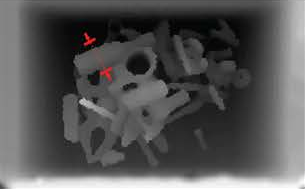
\includegraphics[width=3.2cm]{jeffrey_mahler_d}%
		\subcaption{}%
		\label{subfig:depth_image}%
	\end{subfigure}%
	\end{minipage}%
	%
	\caption{Robot y objetos utilizados en el experimento (imágenes tomadas de \cite{pmlr-v78-mahler17a}).}%
	\label{fig:pmlr-v78-mahler17a}%
\end{figure}
%
El problema de tomar objetos de un contenedor es de gran interés para el presente trabajo, debido a que existen dos formas de aplicar la solución propuesta en este tipo de problemas.
Por un lado, se facilitaría la tarea de tomar un objeto del contenedor, ya que, mediante el algoritmo propuesto, se podrían pre-ordenar los objetos en el contenedor, en un modo que maximice las posibilidades de sujeción de los objetos.
Además, si el problema presenta la tarea adicional de colocar los objetos en otro contenedor, tal como sucede en \cite{8793966}; entonces, se podría volver a aplicar este preordenamiento, de tal forma que la manera de arreglar los objetos en el nuevo contenedor facilite la sujeción posterior de estos.
%
%
% NAMO
%
%
%
\begin{figure}[H]
	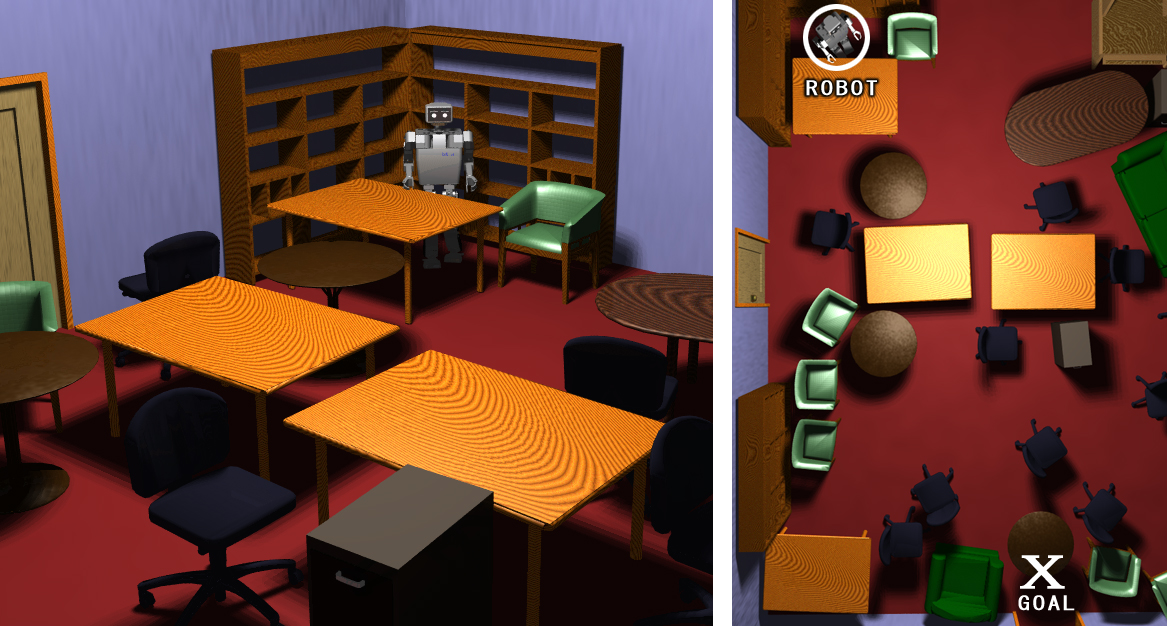
\includegraphics[width=0.9\textwidth]{mike_stilman}%
	\caption{Ejemplo de problema NAMO. El robot debe manipular los objetos que le impiden el paso con el objetivo de trasladarse hacia un lugar específico (imagen tomada de \cite{doi:10.1142/S0219843605000545}).}%
	\label{fig:S0219843605000545}%
\end{figure}
%
En los problemas NAMO uno o varios robots tienen permitido reconfigurar el ambiente donde se encuentran, al mover los obstáculos presentes en él. 
Esto con el objetivo de crear un camino por el cual puedan desplazarse sin mayor dificultad hacia una determinada posición final \cite{doi:10.1142/S0219843605000545}.
En la Figura \ref{fig:S0219843605000545}, se muestra un ejemplo de un problema NAMO encontrado comúnmente en la literatura.

En \cite{doi:10.1177/0278364917739114} se presenta un algoritmo para resolver problemas de planeación de movimientos con un robot humanoide. 
Algunos de estos problemas consisten en situaciones en las que el robot debe realizar tareas de tipo NAMO y/o de reordenamiento de objetos.
Entre estas tareas se puede destacar una en la que, en el entorno navegable por el robot, se encuentra una barrera de pilares manipulables, como se muestra en la Figura \ref{fig:0278364917739114}, los cuales obstaculizan los lugares a los que debe llegar, por lo cual, el robot debe idear un plan para moverlos.

Para cada uno de los problemas se realizaron 50 simulaciones estableciendo un límite de tiempo de 300 segundos.
En sus resultados muestran que, incluir información geométrica en la heurística de su algoritmo es crucial para resolver problemas de manipulación, los cuales involucran restricciones geométricas.
Adicionalmente los autores proponen aplicar su método a tareas de manipulación que involucren variables continuas, así como, incluir acciones para apilar objetos encima de otros.
%
\begin{figure}[H]
	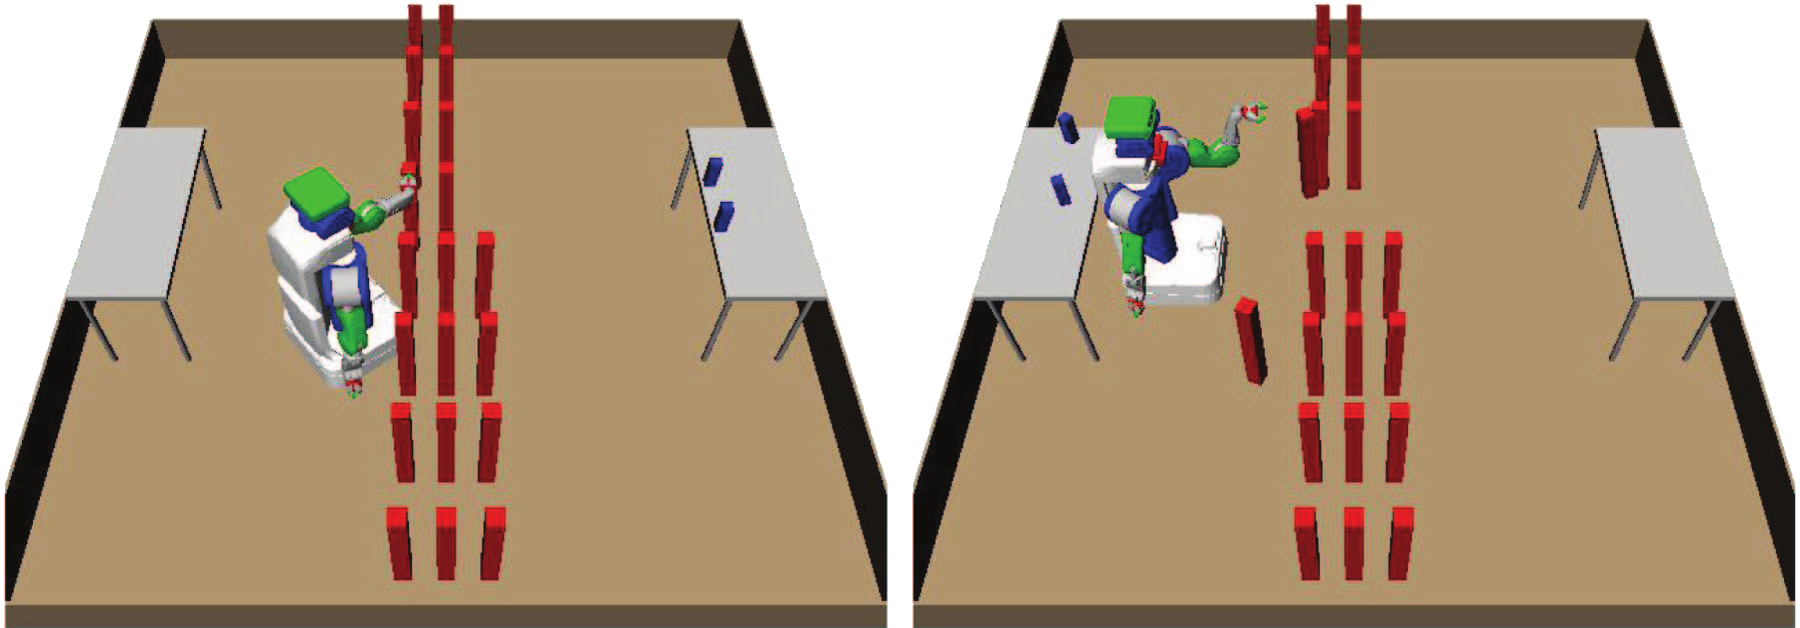
\includegraphics[width=0.95\textwidth]{garrett_caelan_reed}%
	\caption{Ejemplo de una de las tareas que debe llevar a cabo el robot (imagen tomada de \cite{doi:10.1177/0278364917739114}).}%
	\label{fig:0278364917739114}%
\end{figure}
%
En \cite{Kim_Kaelbling_Lozano-Pérez_2019} se plantea resolver algunos problemas que involucran planificación de tareas y movimientos.
Para ello se tiene que establecer una secuencia de movimientos de bajo nivel para un robot (por ejemplo, trasladarse a determinado punto mediante una trayectoria libre de colisiones), con la cual se logre un objetivo de alto nivel (por ejemplo, tomar un objeto).
Esto se logra integrando razonamiento geométrico de bajo nivel con razonamiento simbólico de alto nivel. 
Los autores utilizan un robot humanoide, el cual, junto con una configuración inicial de objetos móviles y obstáculos, debe llegar a una configuración final.

En el trabajo se presenta una nueva forma de representar los estados del mundo mediante un vector de longitud fija.
Los resultados experimentales demuestran que su método es capaz de aprender de una manera más eficiente que los enfoques estándar de aprendizaje por refuerzo, al utilizar menos información durante el entrenamiento.

De forma similar, en \cite{doi:10.1163/156855307782227408} se experimenta con la locomoción autónoma de un robot humanoide en un problema NAMO.
El robot se encuentra en un ambiente que consiste en una habitación con objetos fijos y móviles.
Estos objetos se consideran obstáculos que bloquean el camino para llegar a una posición final, hacia la cual el robot debe trasladarse.
Los obstáculos fijos son representados mediante cajas contenedoras aproximadas, mientras que los móviles se representan mediante modelos de mallas 3D de sillas y mesas, debido a que requieren de un mayor nivel de detalle para poder ser manipulados adecuadamente.

Para lograr su objetivo, el robot percibe y construye un modelo de su ambiente, incluyendo los obstáculos en él.
Con esto elabora una estrategia de navegación para alcanzar la posición objetivo, que consiste en una secuencia de operaciones de desplazamiento y manipulación de los obstáculos.
Los autores consideran que en ambientes con mayor grado de incertidumbre, los robots deben ser capaces de reaccionar a eventos como colisiones no previstas del robot con los obstáculos, así como poder cambiar de decisión acerca de cuál objeto manipular.
Por lo cual, estiman que una mejor integración de la re-planificación y ejecución en problemas NAMO ayudarían a generar tales comportamientos autónomos complejos en robots humanoides.

En \cite{8625041} se presenta un problema NAMO para un brazo robótico.
En este problema, al igual que los problemas NAMO para robots humanoides, se desea que el robot, o más precisamente, su efector final llegue a una posición determinada.
En dicha posición se encuentra un objeto rodeado por varios obstáculos móviles, el cual se desea sujetar; como se muestra en la Figura \ref{fig:8625041}.
Los autores hacen varias simplificaciones al problema, una de las cuales es que, no se consideran obstáculos inmóviles, debido a que se considera que esto generaría efectos de aglomeración entre el robot y los objetos.
La solución que se propone es desplazar los obstáculos con el chasis del brazo hasta llegar al objeto deseado mediante una re-planificación en línea utilizando controles óptimos. 
Esto es, el robot elabora un plan, ejecuta una porción de él, observa el estado resultante y luego re-planifica.
Los resultados muestran que su enfoque conlleva un menor costo, así como un menor tiempo de ejecución que otros enfoques más ingenuos.
Los autores también califican a los trabajos que planifican trayectorias como altamente conservativos y pesimistas.
%
\begin{figure}[H]
	\begin{subfigure}{0.35\linewidth}
		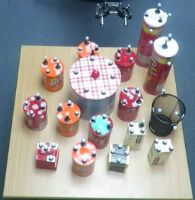
\includegraphics[width=\linewidth]{w_c_agboh_a}%
		\subcaption{}%
		\label{subfig:start_scene}%
	\end{subfigure}%
	%
	\hspace{0.5cm}%
	%
	\begin{subfigure}{0.35\linewidth}
		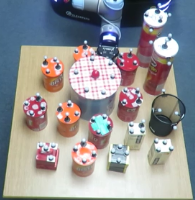
\includegraphics[width=\linewidth]{w_c_agboh_b}%
		\subcaption{}%
		\label{subfig:contact_replaning}%
	\end{subfigure}%
	
	\vspace{3pt}%
	%
	\begin{subfigure}{0.35\linewidth}
		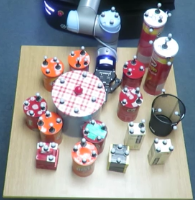
\includegraphics[width=\linewidth]{w_c_agboh_c}%
		\subcaption{}%
		\label{subfig:new_plan}%
	\end{subfigure}%
	%
	\hspace{0.5cm}%
	%
	\begin{subfigure}{0.35\linewidth}
		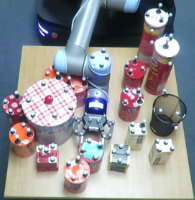
\includegraphics[width=\linewidth]{w_c_agboh_d}%
		\subcaption{}%
		\label{subfig:target_object_grasp}%
	\end{subfigure}%
	%
	\caption{Ejecución del planificador en línea: \subref{subfig:start_scene} escena inicial; \subref{subfig:contact_replaning} el contacto activa la re-planeación; \subref{subfig:new_plan} nuevo plan y \subref{subfig:target_object_grasp} objeto-meta sujetado (imágenes tomadas de \cite{8625041}).}%
	\label{fig:8625041}%
\end{figure}
%
Los problemas NAMO tienen mucha similitud con el problema planteado en este trabajo, esto debido a que, en ambos se tiene como objetivo acceder a una cierta posición en un espacio, con obstáculos en él. 
Particularmente, en el presente caso de estudio, se desea acceder a un objeto rodeado por obstáculos más que a una zona de espacio vacío.
Mientras que en los problemas NAMO se deben re-acomodar los objetos del entorno para llegar a una zona específica, en la presente investigación se busca minimizar el número de acciones necesarias para realizar dicho re-acomodo, con la finalidad de acceder a un objeto obstaculizado más que desbloquear el camino para llegar a una zona específica.

Otra característica de los problemas NAMO es que se enfocan principalmente en los temas de la planificación de movimientos del robot, así como en la planeación de la manipulación de los objetos móviles.
En el trabajo aquí desarrollado se da por hecho que el manipulador puede tomar cualquier objeto, para enfocarse por otro lado en que el entorno imponga las restricciones mínimas para tomarlos.
Esto es, se brinda más atención a asuntos como minimizar las restricciones de sujeción de los objetos en su acomodo inicial, ya que a partir de ello es más probable que las planificaciones de algoritmos NAMO tengan éxito. 
%
%
% MAMO
%
%

Los problemas MAMO son una generalización de los problemas NAMO.
En este dominio, además de las tareas de navegación, el robot requiere remover obstáculos con el objetivo de manipular un objeto, llevándolo desde su posición inicial a una posición final deseada \cite{4209604}.

En \cite{9863895} se presenta un planificador incremental de tareas y movimientos basado en muestreos y grafos jerarquicos, el cual es utilizado por un brazo robótico  para alcanzar objetos \textsl{casi-cilíndricos} (como botellas) inmersos en escenas desordenadas.
Dichas escenas consisten en los objetos cilíndricos colocados en estantes.
El planificador computa un plan para remover obstáculos y generar una trayectoria libre de colisiones para alcanzar el objeto deseado.

Su método consta de dos componentes principales: una planeación de tareas, donde se realiza una expansión incremental de un grafo con la secuencia de obstáculos a remover para alcanzar el objeto meta; y una planeación de movimientos, donde se utiliza otro grafo de estados de colisión, el cual contiene la información de objetos que colisionan con el robot cuando se quiere remover otro objeto.
Mediante este último grafo se corrige y optimiza la secuencia de remociones de objetos-obstáculo para alcanzar el objeto meta.
Esto es, se intenta minimizar el número de obstáculos a ser removidos, optimizando el orden en el que se retiran.

El método además es capaz de lidiar con oclusiones de objetos.
Se demuestra la capacidad de su método para realizar desde tareas simples, hasta movimientos de manipulación complejos, tanto en ambientes reales como virtuales.
Comparado con otros enfoques, su método reduce el tiempo de planeación de tareas y movimientos en un 24.6\!\%.

En \cite{Akbari2019} se aborda el problema de la manipulación de objetos en ambientes desordenados mediante planeación de tareas y movimientos con dos brazos robóticos. 
La idea es que los brazos colaboren para retirar los obstáculos que bloquean un objeto particular hasta tomarlo, tal como se muestra en la Figura \ref{fig:Akbari2019}. 
También se busca un buen lugar donde dejar los obstáculos retirados, para lo cual se utiliza el razonamiento geométrico sobre la colocación de objetos (Figuras \ref{subfig:Akbari2019c} a \ref{subfig:Akbari2019e}). 
Los autores implementan su solución en problemas de tipo MAMO y NAMO.
Aseguran que el principal reto en su investigación fue el proveer al robot la información geométrica de bajo nivel que sirva de guía al planificador de tareas.
Su propuesta fue validada tanto en ambientes virtuales como reales, considerando varias clases de problemas de manipulación de objetos que se encuentran sobre una mesa.
Los resultados muestran que su método es capaz de resolver dichas tareas de manipulación eficientemente, tanto en términos de tiempo de planeación ($16s$, en promedio) como en tasa de éxitos (98\!\%, en promedio), mejorando respecto a otras aproximaciones contra las que se comparan en prácticamente todos los escenarios .
%
\begin{figure}[H]
	\begin{subfigure}{0.3\textwidth}
		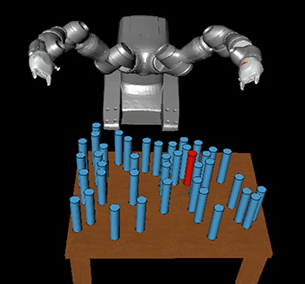
\includegraphics[width=\textwidth]{aliakbar_akbari_a}%
		\subcaption{}%
	\end{subfigure}%
	\hspace{0.25cm}%
	\begin{subfigure}{0.3\textwidth}
		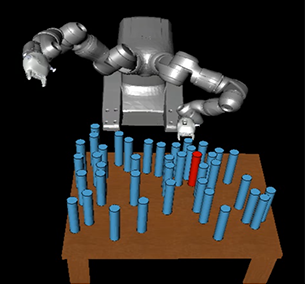
\includegraphics[width=\textwidth]{aliakbar_akbari_b}%
		\subcaption{}%
	\end{subfigure}%
	\hspace{0.25cm}%
	\begin{subfigure}{0.3\textwidth}
		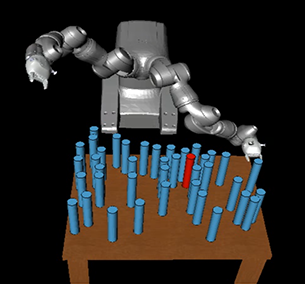
\includegraphics[width=\textwidth]{aliakbar_akbari_c}%
		\subcaption{}%
		\label{subfig:Akbari2019c}%
	\end{subfigure}%
	
	\vspace{3pt}%
	%
	\begin{subfigure}{0.3\textwidth}
		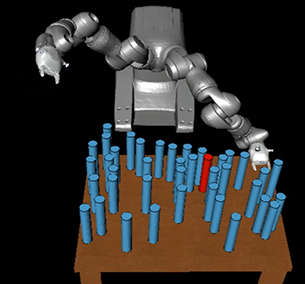
\includegraphics[width=\textwidth]{aliakbar_akbari_d}%
		\subcaption{}%
	\end{subfigure}%
	\hspace{0.25cm}%
	\begin{subfigure}{0.3\textwidth}
		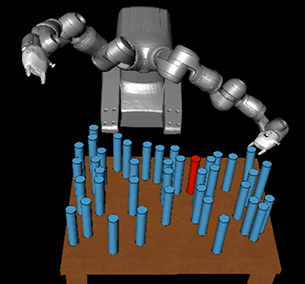
\includegraphics[width=\textwidth]{aliakbar_akbari_e}%
		\subcaption{}%
		\label{subfig:Akbari2019e}%
	\end{subfigure}%
	\hspace{0.25cm}%
	\begin{subfigure}{0.3\textwidth}
		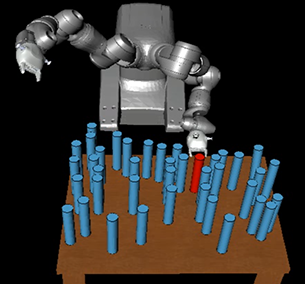
\includegraphics[width=\textwidth]{aliakbar_akbari_f}%
		\subcaption{}%
	\end{subfigure}%
	%
	\caption{Ejecución de un simulador para resolver el problema de manipulación entre objetos desordenados. El robot tiene que sujetar el objeto rojo que se encuentra entre 50 objetos azules (imágenes tomadas de \cite{Akbari2019}).}%
	\label{fig:Akbari2019}%
\end{figure}
%
En el trabajo desarrollado en \cite{4209604} se presenta un algoritmo enfocado en la manipulación planificada, el cual genera planes de manipulación rápidos en un espacio de búsqueda no lineal de dimensión exponencial. 
Para ello se utiliza una búsqueda en profundidad sobre los obstáculos ordenados. 

El plan comienza desde el objeto que se desea tomar (raíz) y a partir de este, se identifican los posibles obstáculos (ramas) sobre los cuales se hace el mismo proceso de forma recursiva.
Se definen tres funciones: \textit{PlanGrasp}, \textit{PlanManipulation} y \textit{PlanNavigation}. 
Si alguna de ellas fracasa, entonces el planificador finaliza la rama actual y hace \textit{backtracking} hasta encontrar una solución o hasta que se agoten las opciones de búsqueda.

En la Figura \ref{fig:4209604} se muestran imágenes de la aplicación de este método en una simulación, donde un robot debe retirar los obstáculos que le impiden tomar un objeto particular.
Los autores realizan pruebas en escenarios con varios objetos, tanto fijos, como móviles y semifijos.
Sus resultados muestran que el $50\%$ del tiempo empleado por todo el proceso es consumido por la función \textit{PlanManipulation}, debido a las constricciones de manipulación de los objetos, así como a que las geometrías de los objetos en estas pruebas son complejas.
%
\begin{figure}[H]
	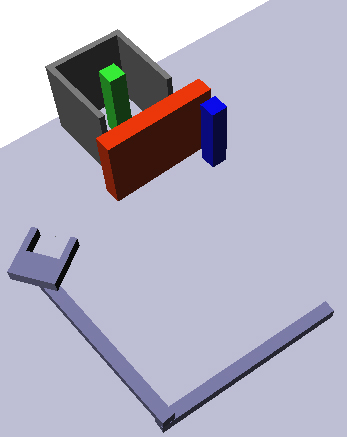
\includegraphics[width=5cm]{m_stilman_a}%
	\hspace{0.5cm}%
	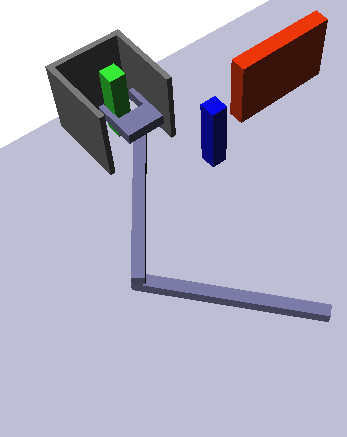
\includegraphics[width=5cm]{m_stilman_b}%
	%
	\caption{Simulación en la que un brazo robótico debe retirar los obstáculos que rodean a un objeto (prisma verde) para posteriormente tomarlo (imágenes modificadas tomadas de \cite{4209604}).}
	\label{fig:4209604}
\end{figure}
%
Al igual que los problemas NAMO, los problemas MAMO se enfocan mayormente en la planeación de movimientos.
Debido a que el objetivo del presente trabajo es encontrar una configuración de objetos que minimice el número de acciones para acceder a alguno de estos, se espera que, por razones muy similares a las explicadas para los problemas NAMO, el algoritmo aquí desarrollado se pueda complementar muy bien con los algoritmos de problemas MAMO. 
%
%
% Problema de reordenamiento
%
%

En el problema de reordenamiento, un robot o manipulador debe moverse en un espacio con objetos en desorden, los cuales debe reordenar en una configuración específica.
Dentro del espacio de trabajo puede haber o no obstáculos, móviles o inmóviles.
Para lograr su objetivo, el robot puede mover los objetos de forma libre, esto es:
%
\begin{enumerate}[label=\alph*)]
	\item De forma no prensil, al empujar los objetos.
	\item De forma prensil, al sujetarlos y trasladarlos de un lugar a otro.
	\item Una combinación de las anteriores.
\end{enumerate}
%
Una de las características que distingue este tipo de problemas de los problemas MAMO, es que la manipulación y re-ubicación se hace sobre varios objetos y no solo sobre uno \cite{2019arXiv190103557H}.
En la Figura \ref{fig:2019arXiv190103557H} se muestra un problema peculiar de este tipo, donde un manipulador debe trasladar dos objetos a zonas determinadas. 
En este caso particular, el orden en que los objetos son trasladados es muy importante, ya que uno obstruye la única trayectoria posible del otro.
%
\begin{figure}[H]
	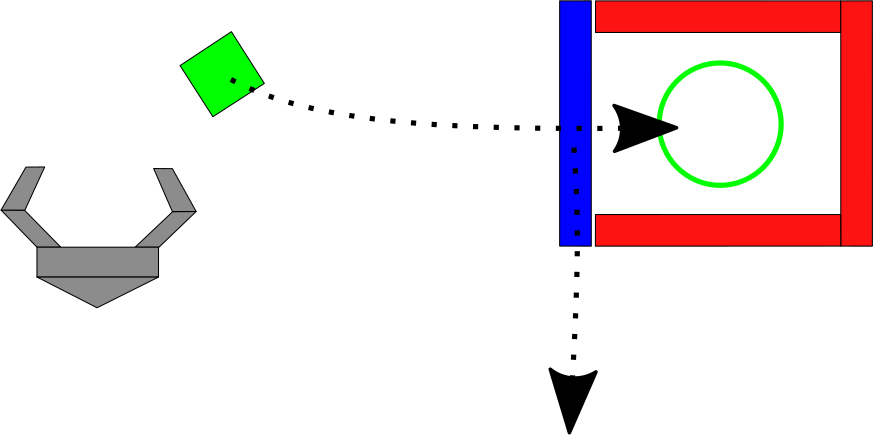
\includegraphics[width = 0.6\textwidth]{joshua_a_haustein}%
	\caption{Problema donde el manipulador debe reconfigurar los objetos, moviéndolos a donde indican las flechas (imagen tomada de \cite{2019arXiv190103557H}).}%
	\label{fig:2019arXiv190103557H}%
\end{figure}
%
En \cite{7487583} se trata el reordenamiento de objetos mediante interacciones no prensiles. 
Los autores proponen un planificador para resolver el problema de la planeación del reordenamiento, que considera dos tipos diferentes de acciones: acciones centradas en los objetos y acciones centradas en el robot.
Las acciones centradas en los objetos guían al planeador a realizar acciones específicas en objetos específicos; mientras que las acciones centradas en el robot mueven al robot sin la intención de manipular un objeto relevante, permitiendo así la interacción simultánea con varios objetos.
Tales interacciones pueden ser el empujar los objetos que obstaculicen otro al cual se quiere llegar, o bien simplemente desplazar un objeto de un lugar a otro, al moverlo entre otros que funcionan como obstáculo.
Se evalúa el planeador en el brazo de un robot humanoide y en un robot móvil de cuatro ruedas diseñado para empujar objetos.
Sus resultados muestran una mejora respecto a otros métodos que solo utilizan un tipo de acción.

En \cite{8462863} se aborda el problema de re-acomodo de objetos de forma no prensil con un robot humanoide; para lo cual se combina un sistema de recompensas con otro de entrenamiento basado en redes $Q$ profundas, los cuales únicamente utilizan información visual, a partir de la cual el robot planea estrategias de re-acomodo. 
Uno de los objetivos de los autores es reducir el número de colisiones con los obstáculos, ya que estas llevan a resultados sub-óptimos.
El sistema de aprendizaje profundo que utilizan consiste en una red convolucional, que recibe como entrada imágenes de los objetos (los cuales tienen forma de cubo) sobre una superficie plana, y da como salida una de cinco direcciones posibles, a lo largo de la cual se debe mover el manipulador para empujar los objetos.
El sistema de recompensas premia al manipulador cuando este se acerca al objeto que debe ser desplazado y lo castiga cuando ocurre alguna colisión.
Los resultados muestran una tasa de éxito de $85\%$ en las tareas asignadas.

De igual forma, en \cite{2018arXiv181010654P} se aborda el problema de reordenamiento de objetos de forma no prensil mediante un brazo robótico de siete grados de libertad, utilizando modelos físicos simples.
En sus configuraciones de objetos se pueden incluir tanto obstáculos móviles como inmóviles.
Un ejemplo de una configuración del robot con los objetos se muestra en la Figura \ref{fig:2018arXiv181010654P}.
Los modelos físicos que se utilizan reducen la dinámica \textit{quasi}-estática a contactos rígidos, lo cual hace que el método empleado sea más rápido y reduce la complejidad del problema.
Sin embargo, al emplear estos modelos de contacto simples y rápidos en las simulaciones, algunas veces estos no imitan lo suficiente la complejidad de los contactos físicos reales; perdiendo en tales ocasiones precisión a cambio de rapidez.
Los resultados experimentales muestran que el método propuesto supera a otras propuestas por un factor de 5 en entornos simulados.
%
\begin{figure}[H]
\begin{tikzpicture}[>=Triangle]
	\node at (0, 0) 
		{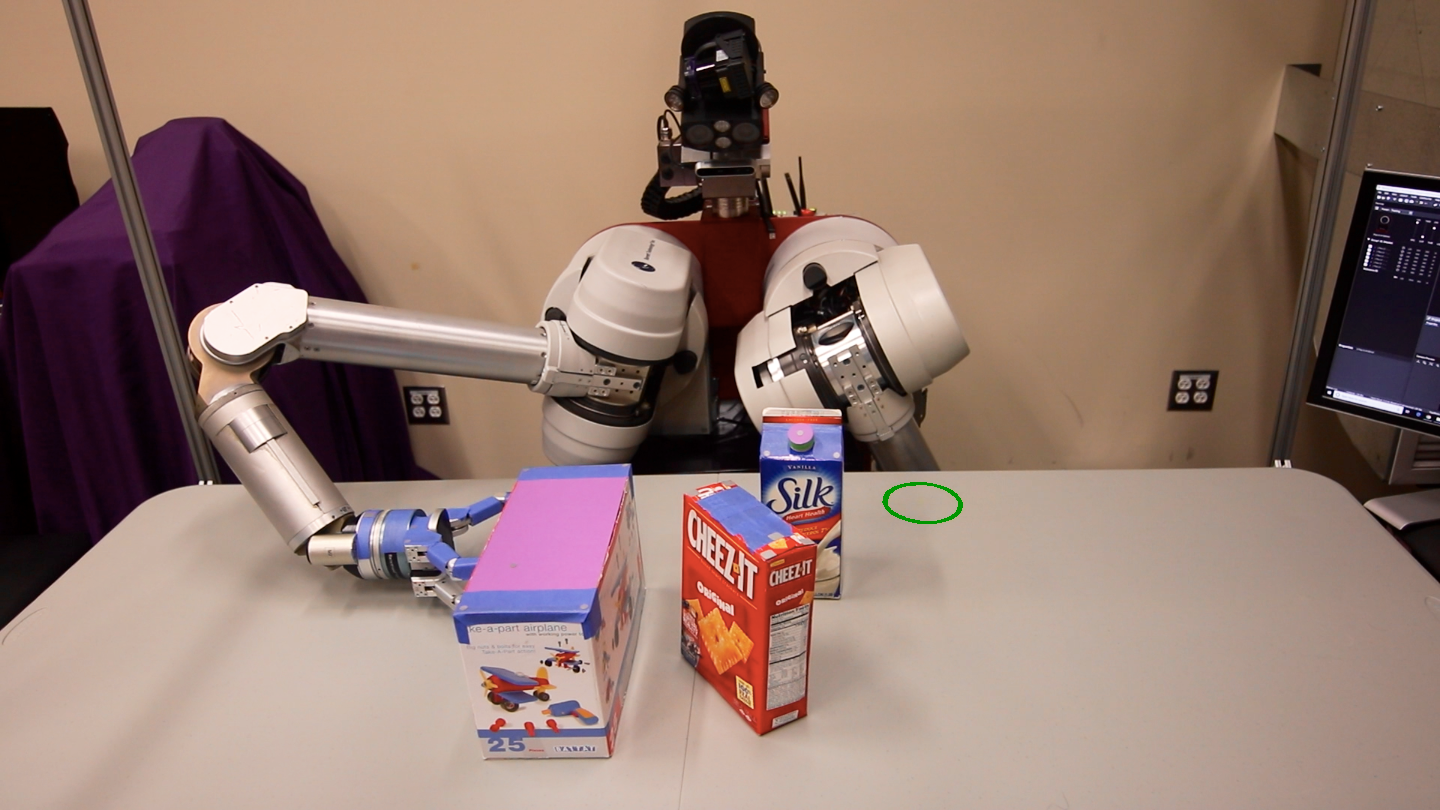
\includegraphics[width = 0.8\textwidth]{lerrel_pinto_a}};
	\node[opacity = 0.4] at (1.8, -0.15) 
		{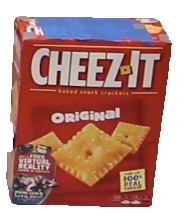
\includegraphics[width = 0.1\textwidth]{lerrel_pinto_b}};
	
	\draw
		[line width = 1.5pt, 
		color = maintextcolor!80, 
		opacity = 0.7] 
		
		[arrows = {-Triangle[width = 4pt, length = 4pt]}] 
		(0.6,-1.6) -- (0.9,-2.3) -- (1.6,-2.3) 
		node[right, maintextcolor, opacity = 1] 
			{\small \textsf{Objetivo}};
	
	\draw
		[line width = 1.5pt, 
		color = maintextcolor!80, 
		opacity = 0.7]
		
		[arrows = {-Triangle[width = 4pt, length = 4pt]}] 
		(1.7, -0.8) -- (2, -1.5) -- (2.6, -1.5) 
		node[right, maintextcolor, opacity = 1] 
			{\small \textsf{Posición meta}};
\end{tikzpicture}
\caption{La meta en este problema de reordenamiento es mover el objetivo a la posición meta deseada (imagen modificada tomada de \cite{2018arXiv181010654P}).}%
\label{fig:2018arXiv181010654P}%
\end{figure}
%
En \cite{7139535} se utiliza un modelador de física embebido, así como un planificador aleatorio para problemas con restricciones cinemáticas y dinámicas, con el objetivo de resolver el problema de re-acomodo de objetos de forma no prensil. 
La principal acción para manipular los objetos es mediante empujes, y una característica destacable es que en el modelado se incluye la posibilidad de tirar los objetos.
Su método está diseñado para que se pueda hacer contacto con cualquier parte del brazo y con varios objetos al mismo tiempo. 
Se define una \textsl{región meta} en la cual se debe colocar el objeto de interés, sin importar la posición final de los demás objetos. 
La comparación de su método con otras soluciones basadas en funciones básicas de movimiento muestra un incremento en la tasa se éxito, mientras que en el tiempo promedio de planificación se observa un incremento con respecto a los otros enfoques.
Como trabajo futuro los autores proyectan incluir más tipos de interacciones entre el manipulador y los objetos, tales como derribar y rodar.

En \cite{10.1007/978-3-030-44051-0_45} se trata el problema de reordenamiento con dos brazos.
En el problema que se aborda, los brazos deben coordinarse para manipular un conjunto de objetos desordenados en una mesa y reordenarlos en una configuración específica, tal y como se muestra en la Figura \ref{fig:10.1007/978-3-030-44051-0_45}.
Los objetos utilizados tienen forma de cubo y los brazos pueden tomarlos por la parte de arriba.
Entre los objetivos principales de la propuesta se encuentra el minimizar el costo del transporte de los objetos cuando estos están siendo re-acomodados, así como evitar colisiones con objetos no manipulados. 
Los autores determinan que los costos involucrados en la solución de su problema son menores al utilizar más de un manipulador. 
Como trabajo futuro proponen explorar casos más generales con $k$ brazos.
%
\begin{figure}[H]
	\begin{subfigure}{0.35\linewidth}
		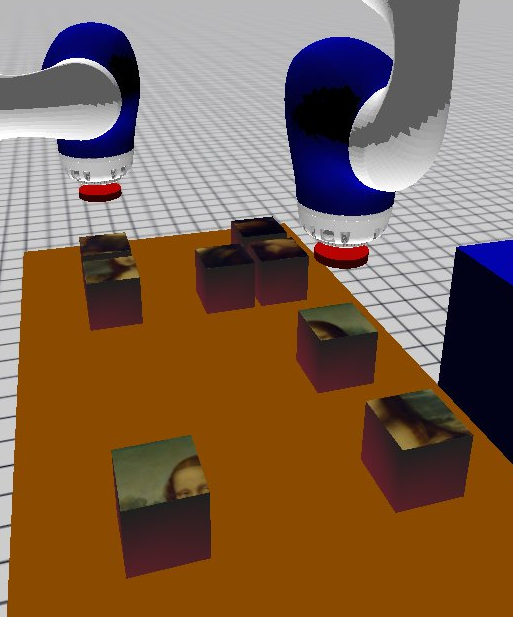
\includegraphics[width = \linewidth]{rahul_shome_a}%
		\label{subfig:initial_conf}%
	\end{subfigure}%
	%
	\hspace{1cm}%
	%
	\begin{subfigure}{0.35\linewidth}
		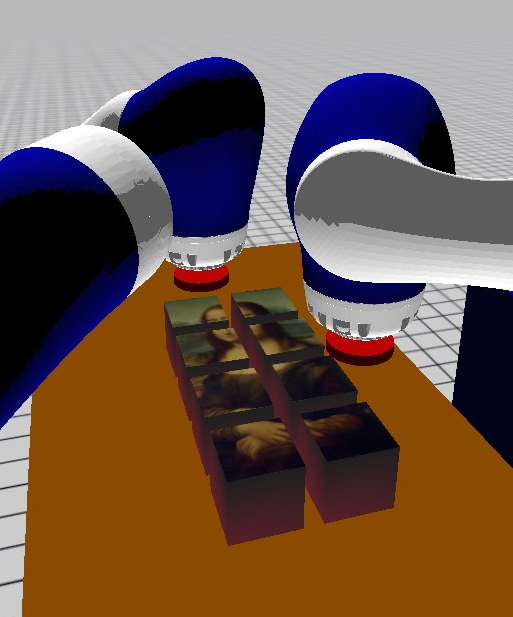
\includegraphics[width = \linewidth]{rahul_shome_b}%
		\label{subfig:final_conf}%
	\end{subfigure}%
	%
	\caption{Ejemplo de re-acomodo de objetos con dos brazos: configuraciones de objetos inicial (izquierda) y final (derecha) (imágenes tomadas de \cite{10.1007/978-3-030-44051-0_45}).}%
	\label{fig:10.1007/978-3-030-44051-0_45}%
\end{figure}
%
De forma distinta, en \cite{2019arXiv190103557H} el reordenamiento de objetos se realiza mediante acciones no prensiles con cualquier parte de un brazo robótico.
El robot debe re-acomodar algunos objetos que se encuentran entre obstáculos en una superficie plana.
Se presenta un algoritmo eficiente de planeación que está diseñado para trabajar con poca información acerca de las habilidades de manipulación del robot, por lo cual, sus creadores aseguran que dicho método es fácilmente adaptable a diferentes arquitecturas de manipuladores.
Sin embargo, el hacer que el algoritmo sea agnóstico a las características del manipulador puede llevar a que exista una alta probabilidad de falla, debido a predicciones imprecisas.
Los autores afirman que un reto mayor en este tipo de problemas es la necesidad de retirar obstáculos, lo cual requiere de un nivel más alto de lógica. 
Sus resultados muestran que su algoritmo supera por un factor mayor a dos a otros enfoques de la literatura en lo que al tiempo de planeación se refiere.

Una diferencia importante de este tipo de problemas con el planteado en este trabajo es el hecho de que se conoce la configuración a la que se debe llegar (al contrario de problemas como el del contenedor).
Sin embargo, uno de los trabajos en el tema del reordenamiento que tiene algunas similitudes con el presente es \cite{Han-RSS-17}.
En él se trata de reordenar, mediante un manipulador prensil, un conjunto de objetos en una superficie plana, los cuales son tomados desde la parte de arriba por dicho manipulador, como se puede apreciar en la Figura \ref{fig:Han-RSS-17}. 
La similitud recae en que se busca minimizar el número de acciones \textsl{tomar-dejar}, ya que, debido a la presencia de obstáculos en las posiciones finales, en ocasiones hay que dejar los objetos en posiciones intermedias antes de colocarlos en su posición final.
%
\begin{figure}[H]
	\begin{subfigure}{0.1978\linewidth}
		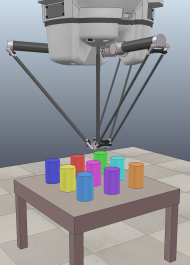
\includegraphics[height=118pt]{shuai_han_a}%
		\subcaption{}%
		\label{subfig:manipulator_objects}%
	\end{subfigure}%
	\hfill%
	\begin{subfigure}{0.3783\linewidth}
		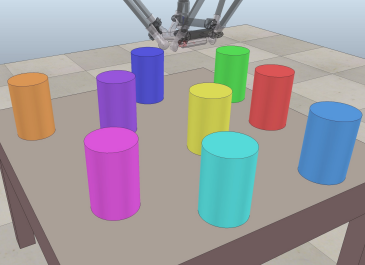
\includegraphics[height=118pt]{shuai_han_b}%
		\subcaption{}%
		\label{subfig:initial_arrangement}%
	\end{subfigure}%
	\hfill%
	\begin{subfigure}{0.3941\linewidth}
		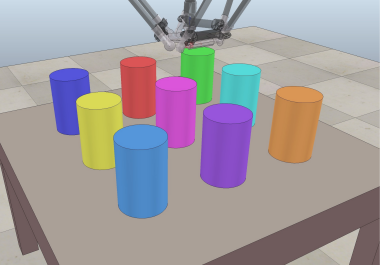
\includegraphics[height=118pt]{shuai_han_c}%
		\subcaption{}%
		\label{subfig:final_arrangement}%
	\end{subfigure}%
	%
	\caption{Vista de \subref{subfig:manipulator_objects} manipulador y los objetos, así como de las configuraciones \subref{subfig:initial_arrangement} inicial y \subref{subfig:final_arrangement} final de los objetos (imágenes tomadas de \cite{Han-RSS-17}).}%
	\label{fig:Han-RSS-17}%
\end{figure}
%
Como recordatorio, en el presente trabajo se busca crear un arreglo de objetos que minimice el número de acciones para tomar un objeto, tomando en cuenta sus restricciones de agarre. 
Donde cada acción consiste en retirar un obstáculo que impida, directa o indirectamente, la sujeción del objeto deseado.

Cabe destacar que ninguno de los trabajos mencionados aborda de manera precisa el problema propuesto, por lo cual no es posible una verdadera comparación entre las investigaciones mencionadas y la presente.
Asimismo, hasta la fecha no se conoce una investigación que proponga una solución al problema aquí planteado.